\section{Efficiency}

The goal of PIX is to provide a toolkit that enables the construction of
instrumentation tools that produce an efficient instrumented
executable. Specifically PIX is designed to provide efficiency when
the number of instrumentation points is large since cases where the number of
instrumentation points is high are the cases where inefficient instrumentation
has the largest negative impact on application performance. 
In this section we describe some of the important mechanisms used by PIX 
to produce efficient instrumented code.

\label{Subsection:Relocation}
\subsection{Code Relocation}
The use of relocation at the function level in PIX stems from the fact
that instrumentation is being performed statically on a platform that uses a
variable-length instruction set. Because of the variable-length length instructions, it may not always be possible to instrument
an arbitrary point in the executable due to the lack of space for a jump instruction large enough to reach the instrumentation code. 
A typical strategy used by static instrumentation toolkits on platforms with fixed-length instruction sets is to
replace a single instruction at the instrumentation point with a
branch instruction that will transfer control to the instrumentation code. This is fairly straightforward because, by the
definition of a fixed-length instruction set, the instruction being replaced and
the replacing jump instruction have the same length. 
In x86 platforms, a jump instruction that uses a 32-bit offset requires 5 bytes. However, for some
instrumentation points of interest there may not be enough space to hold a 5 byte
jump instruction because the instrumentation point itsself (which might be an instruction or a
basic block) is smaller than 5 bytes. 

Figure \ref{Figure:InstructionSizes} shows a breakdown of the sizes of
instructions for many of the SPEC CPU2000 Integer benchmarks. This figure shows that for these benchmarks,
between 52\% and 74\% of instructions are smaller than 5 bytes. In fact an average of 64\% of instructions
are smaller, which indicates that the the generic technique of replacing 
an instruction with a branch to instrumentation code deserves reexamination because without modification
this technique cannot provide instrumentation to large portions of the application code, which becomes
especially untenable if the instrumentation tool requires many instrumentation points.

\begin{figure}[ht]
\centering
\label{Figure:InstructionSizes}
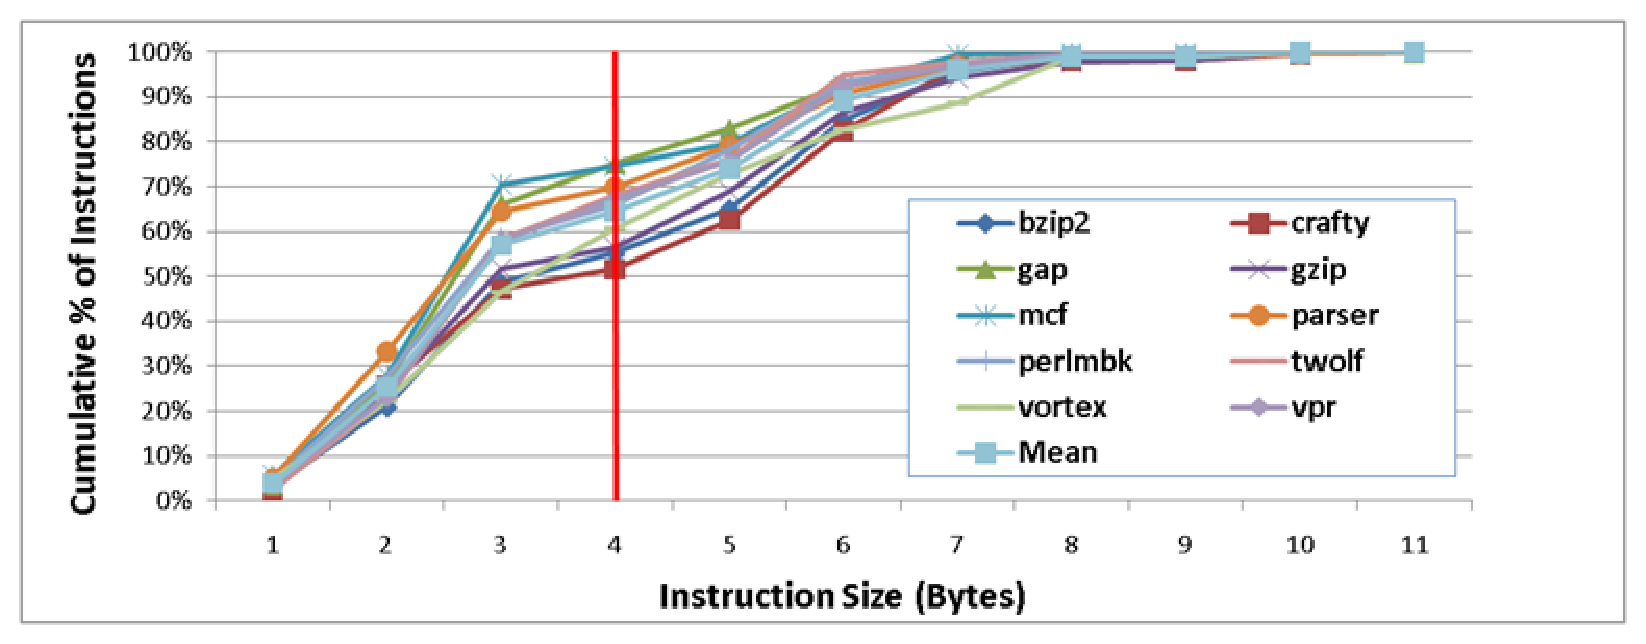
\includegraphics[scale=0.5]{instsize.eps}
\caption{Instruction sizes for several benchmarks presented in a cumulative basis.}
\end{figure}

This leaves two options for transferring control to the instrumentation code.
Either a technique entirely distinct from the idea of using a single
unconditional branch to execute the control transfer must be used or somehow the application code must be altered
in such a way that it can accommodate a single large control instruction that is larger than
the original amount of space available at the instrumentation point. One alternative
technique for transferring control flow to an arbitrary point in the program could be to use a series of branches,
where the instruction at the instrumentation point is a small branch that
transfers control to a larger intermediate branch. This
method is unsatisfactory because the smallest traditional branch instruction available
on the x86 platform is 2 bytes in length, yet there are
instrumentation points with only a single byte available to them. Referring again to figure \ref{Figure:InstructionSizes}, we see
that an average of 4\% of instructions use only a single byte.
Besides, this technique would require additional space to be available in close proximity to the instrumentation points since these
smaller 2-byte branches are also very short reaching. 

%There will also be some overhead associated with setting up a stack frame for the instrumentation function. 
Another option is the method proposed by the BIRD project \cite{nanda2006bird}, which
proposes the use of the single-byte \begin{it}INT3\end{it} instruction when a larger traditional
branch does not fit at the instrumentation point. This instruction is functionally
perfect for static instrumentation because it consumes only a single byte and
allows us to transfer control to an arbitrary location by using the exception handling
facilities provided by the system. We performed a cursory study on this scheme
from an efficiency standpoint to determine whether it was worth further
investigation. On a small benchmark set, our implementation of using
\begin{it}INT3\end{it} only when 5 byte branches do not fit at
the instrumentation point introduces slowdown of at least 100X for
even the simple task of counting the number of executions of each basic block in the code. As one might
expect, this mechanism is unsuitable for efficient instrumentation since the
heavyweight system call conventions are being invoked on a fairly regular basis to
transfer control from the application to the instrumentation code.

In PIX, we use reorganization of the code at the function level so that
there is enough space at every instrumentation point to accommodate a 5 byte
jump. Specifically, the steps used by PIX to relocate the functions and prepare them
for instrumentation are as follows:

\begin{enumerate}
 \item \textit{Function Displacement + Entry Point Linking}
 \item \textit{Branch Conversion}
 \item \textit{Instruction Padding}
 \item \textit{Instrumentation}
\end{enumerate}

Figure \ref{Figure:Relocation} shows an example of this process performed on 
a simple example function in order to prepare the function for instrumentation
that will be inserted at every basic block.

\begin{figure}[ht]
\centering
\caption[Optional caption for list of figures]
{The steps taken in order to prepare a function for instrumentation that will
be inserted at every basic block.}
\subfigure[An unmodified application function.]{
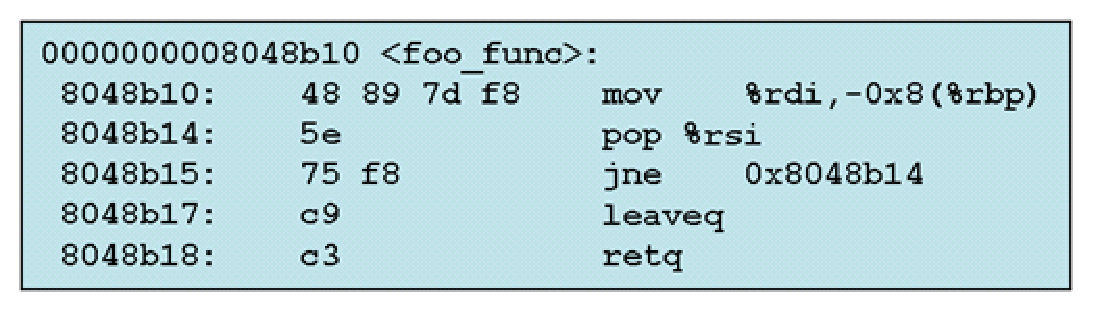
\includegraphics[scale=0.38]{funcp1.eps}
\label{Figure:funcp1}
}
\subfigure[The application function after it has been relocated and the old function entry has been linked to it.]{
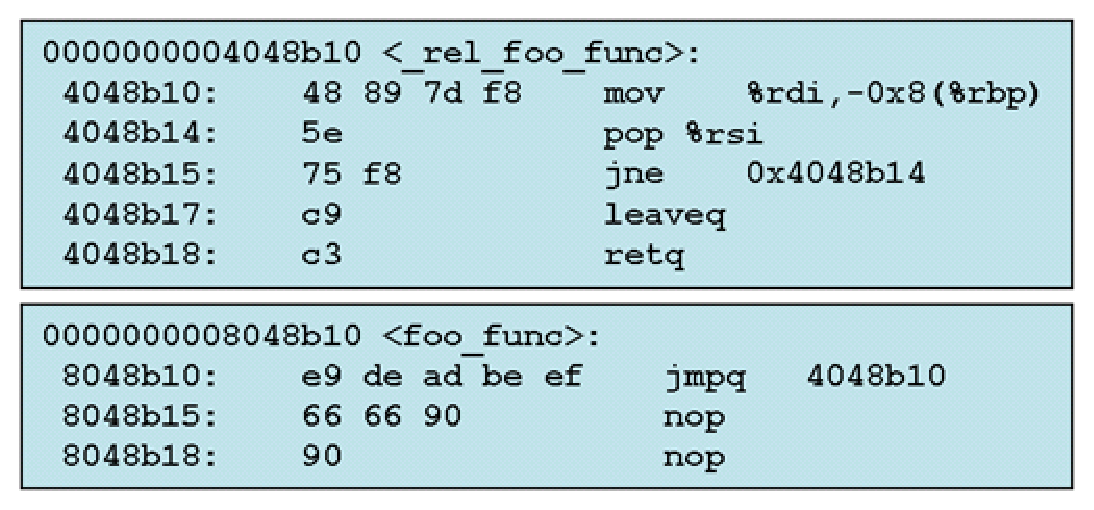
\includegraphics[scale=0.38]{funcp2.eps}
\label{Figure:funcp2}
}
\subfigure[The application function after the branch has been converted to use a 32-bit offset.]{
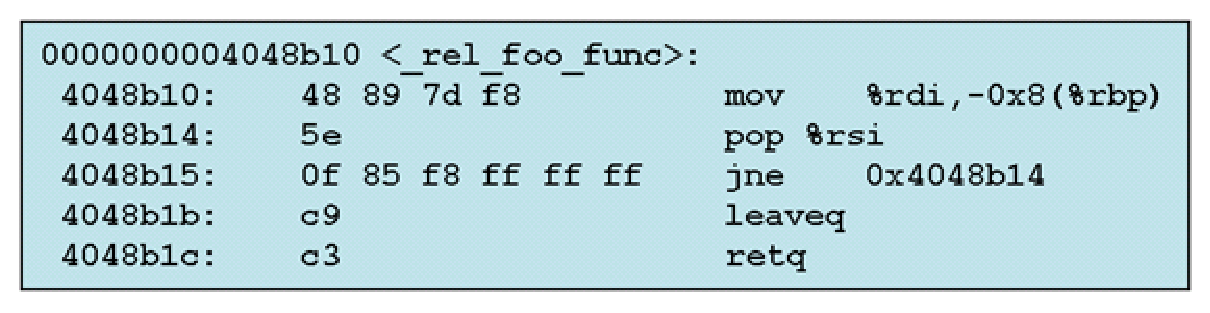
\includegraphics[scale=0.38]{funcp3.eps}
\label{Figure:funcp3}
}
\subfigure[The application function after it has been padded with nop instructions so that each basic block
is large enough to hold a 5 byte jump instruction.]{
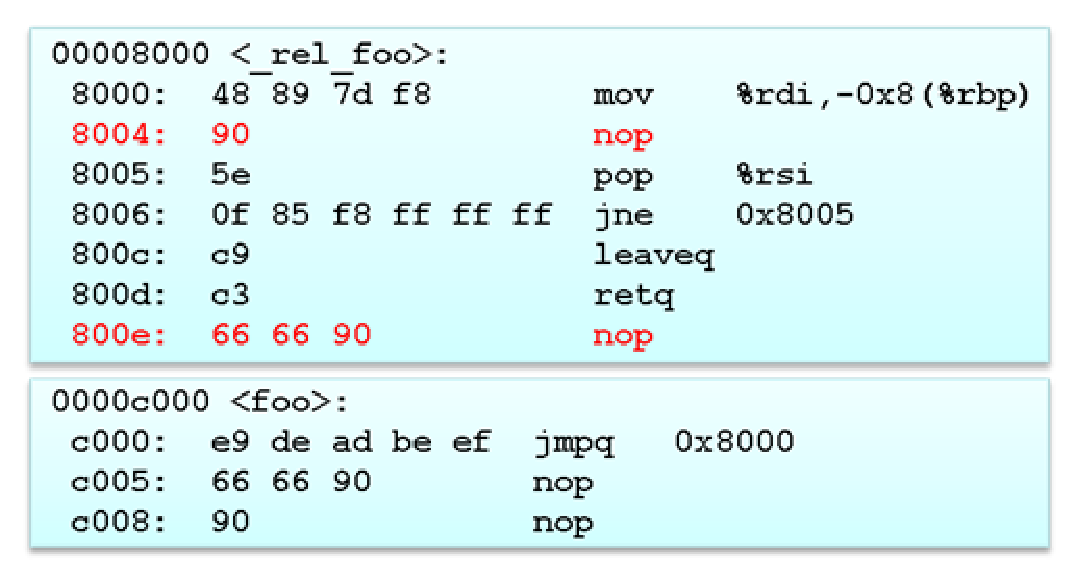
\includegraphics[scale=0.38]{funcp4.eps}
\label{Figure:funcp4}
}
\subfigure[The application function after a single basic block (Basic Block 1) has been instrumented.]{
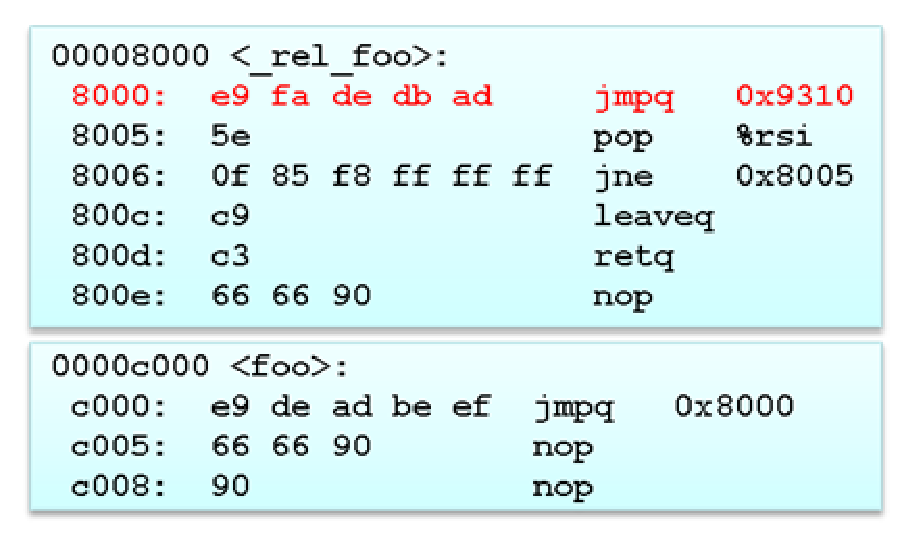
\includegraphics[scale=0.38]{funcp5.eps}
\label{Figure:funcp5}
}
\label{Figure:Relocation}
\end{figure}


Figure \ref{Figure:funcp1} shows a function body prior to any relocation/instrumentation activities.
\textit{Function Displacement + Entry Point Linking} relocates the contents of the entire function to an area of the text section allocated
for the instrumentation. This is done because functions are often packed tightly together. As a result it is generally not possible to keep a function's entry point and
expand its size without disturbing the entry point of another nearby function. The original entry point of the function is then linked to the new location
of the function body by placing an unconditional branch there that transfers control to the new relocated function entry point. 
Linking is done in this fashion because most references to the entry point of a function are in the form of function calls, which
routinely are indirect references (i.e. their value is computed or looked up at runtime) and are difficult to resolve
prior to runtime. See figure \ref{Figure:funcp2}. \textit{Branch Conversion}, shown in figure \ref{Figure:funcp3}, 
converts each short conditional branch in the relocated function to the equivalent
5-byte branch instruction. Since the code is being reorganized in the next step, which may strain the limits of
smaller 8-bit or 16-bit offsets, we convert all branches to use 32-bit offsets so that the targets of each branch
will still be reachable without having the need to make furter changes to the code. Note that there may be some opportunity
here to reduce space by using the smallest branch offset size that accommodates the branch, but currently a single 
unified technique is used in this case to simplify the implementation. Our experiments in Section \ref{Section:Results}, 
however, indicate that the opportunities for improving efficiency for this technique are minimal. \textit{Instruction Padding}, seen
in figure \ref{Figure:funcp4}, pads
each instrumentation point with \begin{it}nop\end{it} instructions so that a 5 byte branch can be accomodated. \textit{Instrumentation} replaces the
some instructions at each instrumentation point with a jump that transfers control to the instrumentation code, which is shown in figure
\ref{Figure:funcp5}.

There are several ways that whole function relocation may adversely affect 
the performance of the instrumented executable independent of the overhead
that will be imposed by the additional instrumentation code. Each function call
now has an extra control interruption associated with it since control must be passed first to the original function entry
point and then to the redirected to the relocated function entry point. In addition it is possible that using 32-bit offsets for every branch rather than
some smaller number of bits has an overhead associated with it. Since the code is being reorganized and expanded, 
we might destroy some positive alignment and size optimizations that the compiler might have made on the instructions in the
function. And finally our technique introduces extra instructions to be executed in the form of nops.

To quantify the impact that function relocation and the other organizational changes have
on the performance of applications, we show the results of experiments
where we generated executables in which functions are relocated, branches are converted to use 32-bit offsets, and 
instruction padding is applied. These experiments show the overhead of the transformations applied to the executable 
in order to prepare it for instrumentation but before any instrumentation code is inserted. The overhead on a set of ten of the 
SPECINT 2000 benchmarks never exceeds 6.5\%, with an average
overhead of just 1.6\%. Thus the basic overhead incurred by the code reorganization in PIX to accomodate all instrumentation points is
well within reason and does not represent a major hurdle for efficiency of the instrumented code.

\subsection{Efficient Instrumentation Snippets}

In most instrumentation tools, the tasks performed by the instrumentation tool are accomplished by allowing the user
to transfer control from instrumentation points in the application to instrumentation functions provided by the user, typically
via a shared library or some object code. Since these instrumentation functions are delivered via a shared library or other
object code, the instrumentation tool developer has the advantage of being able to use a software devlepment toolchain and can
write the code in a language that compiles to the underlying object code. However, such a delivery mechanism is heavyweight due to 
the overhead of a function invocation including saving the complete machine state for all possibles cases in the instrumentation function. In cases where
efficiency is important, it can be more desirable to insert small sequences of assembly code to perform a task and only
save the small subset of machine state that will be affected rather than relying entirely on more heavyweight instrumentation functions and the
more costly state preservation that comes with it.

Some of this state preservation comes in the form of protecting the application call stack from the use of
the call stack by the instrumentation function. The call stack requires protection from the 
instrumentation code during execution because compilers will often optimize a leaf function
by not explicitly creating a stack frame for the local function data to operate in. This optimization is safe for the application because during its
normal execution a leaf function will never call another function and thus its errant stack contents can never be smashed. In the case of an instrumentation
tool that calls an instrumentation function from a leaf, this guarantee no longer holds. Thus, the area above the stack needs to be protected when
an instrumentation function is called from a leaf function. During the disassembly of a function, PIX notes whether it is a leaf function (i.e. whether it contains any call
instructions). Later, during instrumentation, it automatically protects the stack contents for any instrumentation function calls that are made by
incrementing the stack pointer by a fixed safe amount, which has the effect of giving the leaf function a large stack frame while the instrumentation
function's stack frame uses the stack.

Consider the example of an instrumentation point where the desired outcome is to increment a counter that resides in memory. 
In order to accompish this task with an instrumentation snippet, control is transferred to the
instrumentation point's trampoline which will save the platform's flags register, update the counter in memory, restore
the flags register, then transfer control back to the application. Using an instrumentation function, prior to performing
the task the trampoline must save the flags register, any registers used by the function, and
possibly perform some form of stack protection.
It also requires at least 2 more control transfers to enter and exit the instrumentation function. 
Furthermore these control flow transfers generally use the call/return paradigm, which in addition to changing the
application's program counter will also store and retreive information about the function call site onto the stack. 

The use of the instrumentation function is also more likely to pollute the instruction cache more than using a compact
instrumentation snippet. For an instrumentation snippet the application code must contend with the trampoline code
only, whereas using an instrumentation function puts the function code into contention with the other two as well. Hence 
instrumentation functions tend to be more heaviweight than instrumentation snippets. Using snippets rather than functions 
whenever possible allows us to more efficiently gather 
\textit{asynchronous} program information, which intuitively can be thought of as any information that could be dumped to
disk and processed offline. Gao et. al. \cite{gao2005aliter} demostrate that using lightweight instrumentation snippets 
to buffer information which is later processed by more heavyweight instrumentation functions in batches is an efficient
yet entirely lossless way of processing asynchronous program information. The avaialability of instrumentation 
snippets gives tool developers the flexibility to choose either snippets or functions
depending on their performance goals and software engineering needs.
